%This work is licensed under the Creative Commons
%Attribution-ShareAlike 4.0 International License. To view a copy of
%this license, visit http://creativecommons.org/licenses/by-sa/4.0/ or
%send a letter to Creative Commons, PO Box 1866, Mountain View, CA
%94042, USA.

\documentclass[twoside,openright,titlepage,fleqn,
	headinclude,12pt,a4paper,BCOR5mm,footinclude
	]{scrbook}
%\documentclass[a4paper,11pt]{book}
\usepackage[utf8]{inputenc}
%\usepackage[latin1]{inputenc}
\usepackage{lmodern}
\usepackage{microtype}
\usepackage[T1]{fontenc}
\usepackage{makeidx}
%\usepackage[italian]{babel}
%\usepackage{graphicx}
\usepackage{lscape}
\usepackage{siunitx}
\usepackage{enumitem}
\usepackage{subfiles}
\usepackage{listings}
\usepackage{algorithm}
\usepackage{algpseudocode}
%\usepackage{pgf}
\usepackage{xparse}
\usepackage{float}
\usepackage{color}
%\usepackage{xcolor}

%pacchetti del modello per la tesi
%--------------------------------------------------------------
\usepackage[square,numbers]{natbib} 
\usepackage[fleqn]{amsmath}  
\usepackage{dia-classicthesis-ldpkg} 
\usepackage{mathtools}
\usepackage{amsfonts}
\usepackage{amssymb}
\usepackage{amsthm}
\usepackage{pifont}
% Options for classicthesis.sty:
% tocaligned eulerchapternumbers drafting linedheaders 
% listsseparated subfig nochapters beramono eulermath parts 
% minionpro pdfspacing
\usepackage[eulerchapternumbers,subfig,beramono,eulermath,
	parts]{classicthesis}
%--------------------------------------------------------------
\usepackage{tikz}
\usetikzlibrary{shapes, chains, scopes, shadows, positioning, arrows,
  decorations.pathmorphing, calc, mindmap, petri}

\usepackage{cleveref}
\usepackage{acronym}

%comandi per modello
%--------------------------------------------------------------
\newcommand{\myTitle}{B-Spline methods for designing smooth spatial
  paths with obstacle avoidance\xspace}
\newcommand{\mySubtitle}{Metodi B-spline per disegnare percorsi
  regolari in ambienti tridimensionali contenenti ostacoli}
\newcommand{\mySubsubtitle}{Tesi di Laurea Magistrale in Informatica}
% use the right myDegree option
\newcommand{\myDegree}{Corso di Laurea Magistrale in Informatica \xspace}
\newcommand{\myName}{Stefano Martina\xspace}
\newcommand{\myMail}{stefano.martina@stud.unifi.it}
\newcommand{\myProf}{Alessandra Sestini\xspace}
%\newcommand{\myOtherProf}{Carlotta Giannelli\xspace}
\newcommand{\mySupervisor}{Carlotta Giannelli\xspace}
\newcommand{\myFaculty}{Scuola di Scienze Matematiche Fisiche e Naturali\xspace}
\newcommand{\myDepartment}{
	Department of mathematics and computer science\xspace}
\newcommand{\myUni}{\protect{
	Universit\`a degli Studi di Firenze}\xspace}
\newcommand{\myLocation}{Firenze\xspace}
\newcommand{\myAcademicYear}{2015/2016\xspace}
\newcommand{\myMonth}{Luglio\xspace}
\newcommand{\myYear}{2016\xspace}
\newcommand{\myVersion}{Version 0.1\xspace}
\newcommand{\mycopyright}{
  this work is licensed under a
  \href{http://creativecommons.org/licenses/by-sa/4.0/}{Creative
    Commons Attribution-ShareAlike 4.0 International License 
\includegraphics[width=1cm]{logo/logoCC.png}}\xspace}
\newlength{\abcd} % for ab..z string length calculation
% how all the floats will be aligned
\newcommand{\myfloatalign}{\centering} 
\setlength{\extrarowheight}{3pt} % increase table row height
\captionsetup{format=hang,font=small}
%--------------------------------------------------------------
% Layout setting
%--------------------------------------------------------------
\usepackage{geometry}
\geometry{
	a4paper,
	ignoremp,
	bindingoffset = 1cm, 
	textwidth     = 13.5cm,
	textheight    = 21.5cm,
	lmargin       = 3.5cm, % left margin
	tmargin       = 4cm    % top margin 
}
%--------------------------------------------------------------

%comando per impostazioni float di default
\makeatletter
\def\fps@figure{!htbp}
\def\fps@table{!htbp}
\def\fps@code{!htbp}
\makeatother

%cambia comportamento delle description
\renewcommand{\descriptionlabel}[1]{\hspace{2em}\hspace{\labelsep}\textbf{#1}}


%definisce un nuovo ambiente float per il codice
\newfloat{code}{!htbp}{}
\floatname{code}{Codice}

%comando per dimensioni testo
\newcommand{\dimg}{\tiny}
\newcommand{\codg}[1]{\dimg \unicocodet{#1}}
%  \lstinline[basicstyle=\dimg\ttfamily\bfseries,breaklines=true]|#1|


\newcommand{\dims}{\scriptsize}
\newcommand{\cods}[1]{\dims\unicocodet{#1}}
%  \lstinline[basicstyle=\dims\ttfamily\bfseries,breaklines=true]|#1|

%comando per inserire un link
\newcommand{\link}[1]{\unicocode{#1}}


%comando per inserire un file
\newcommand{\file}[1]{\unicocode{#1}}

\newcommand{\bigO}{\ensuremath{\mathcal{O}}}

\def\transW{8mm}
\def\transH{2mm}

\tikzstyle{figureFrame}=[rectangle, rounded corners=2pt, inner sep = 0.3cm, drop shadow, draw=black!50, fill=white, anchor=south west, inner sep=0]
\tikzstyle{imageLabel}=[text=red]
\tikzstyle{imageArrow}=[draw=red, line width=0.5mm, ->]
\tikzstyle{obstacle}=[fill=yellow!50, draw=black]
\tikzstyle{convexHull}=[fill=blue!30]
\tikzstyle{convexHullBord}=[color=black, dotted]%dash pattern=on 3pt off 3pt]
\tikzstyle{knot}=[color=red, draw=black]
\tikzstyle{knotPoly}=[color=black, line width=0.25mm]
\tikzstyle{controlToKnot}=[color=black, dotted]
\tikzstyle{controlPoly}=[color=black, line width=0.25mm]
\tikzstyle{controlPolyHigh}=[color=red, line width=0.25mm]
\tikzstyle{controlPolyTract}=[color=black, line width=0.25mm, dash pattern=on 3pt off 3pt]
\tikzstyle{controlPolyTractHigh}=[color=red, line width=0.25mm, dash pattern=on 3pt off 3pt]
\tikzstyle{obstacleTract}=[draw=black, line width=0.25mm, dash pattern=on 3pt off 3pt]
\tikzstyle{spline}=[color=red, line width=0.5mm]
\tikzstyle{controlVert}=[color=green, draw=black]
\tikzstyle{controlVertHigh}=[color=red, draw=black]
\tikzstyle{obstaclePoint}=[color=red, draw=black]
\tikzstyle{site}=[color=blue, draw=black]
\tikzstyle{siteHigh}=[color=red, draw=black]
\tikzstyle{textArrow}=[draw=red, line width=0.5mm, ->]
\tikzstyle{vertex}=[color=green, draw=black]
\tikzstyle{vertexHigh}=[color=red, draw=black]
\tikzstyle{intersection}=[color=red, draw=black]
\tikzstyle{poly}=[color=black, line width=0.25mm]
\tikzstyle{polyTract}=[color=black, line width=0.25mm, dash pattern=on 3pt off 3pt]
\tikzstyle{cutting}=[color=red, line width=0.25mm]

\colorlet{mmcb}{black!70}
\colorlet{mmc1}{red!80}
\colorlet{mmc2}{blue!80}
\colorlet{c1}{green!20}
\colorlet{c2}{blue!10}
\colorlet{c3}{yellow!10}
\colorlet{c4}{red!10}
\colorlet{drawColor}{black!80}
\colorlet{commentColor}{green!70!black!90}
\colorlet{codeBgColor}{yellow!50}
\colorlet{bashBgColor}{green!50}

\tikzset{onslide/.code args={<#1>#2}{%
  \only<#1>{\pgfkeysalso{#2}} % \pgfkeysalso doesn't change the path
}}
\tikzset{temporal/.code args={<#1>#2#3#4}{%
  \temporal<#1>{\pgfkeysalso{#2}}{\pgfkeysalso{#3}}{\pgfkeysalso{#4}} % \pgfkeysalso doesn't change the path
}}

\tikzstyle{alertStar}=[circle, decorate, decoration={zigzag,segment length=3.12mm,amplitude=1mm}, align=center, drop shadow, draw=drawColor, fill=white]
\tikzstyle{oval}=[ellipse, align=center, drop shadow, draw=drawColor, fill=white]
\tikzstyle{rect}=[rectangle, rounded corners=2pt, align=center, drop
shadow, draw=drawColor, fill=white]
\tikzstyle{arrow}=[->, very thick, >=stealth', draw=black!80]
\tikzstyle{myMindmap}=[mindmap,
every node/.style={concept, minimum size=5mm, text width=5mm}, 
% every child/.style={level distance=10mm, concept color=mmcb}
level 1/.append style={level distance=10mm,sibling angle=45},
level 2/.append style={level distance=10mm,sibling angle=45},
level 3/.append style={level distance=10mm,sibling angle=45}
]
\tikzstyle{myPlace} = [place, very thick, draw=drawColor, fill=white, drop shadow]
\tikzstyle{transExpH} = [transition, very thick, draw=drawColor, fill=white, drop
shadow, minimum width=\transW, minimum height=\transH]
\tikzstyle{transExpV} = [transition, very thick, draw=drawColor, fill=white, drop
shadow, minimum width=\transH, minimum height=\transW]
\tikzstyle{transDetH} = [transition, very thick, draw=drawColor, fill=black, drop shadow, minimum width=\transW, minimum height=\transH]
\tikzstyle{transDetV} = [transition, very thick, draw=drawColor, fill=black, drop shadow, minimum width=\transH, minimum height=\transW]
\tikzstyle{pre}=[<-, very thick, >=stealth', draw=drawColor]
\tikzstyle{preN}=[<-, very thick, >=o, draw=drawColor]
\tikzstyle{post}=[->, very thick, >=stealth', draw=drawColor]
\tikzstyle{highlight}=[draw=red]

\NewDocumentEnvironment{myfig}{mm}{
  \begin{figure}
    \begin{center}
    }{
    \end{center}
    \caption{#1}
    \label{#2}
  \end{figure}
}

%comando per inserire una immagine
\NewDocumentCommand{\image}{mmmo}{
  \begin{figure}
    \begin{center}
      \begin{tikzpicture}
        \node [figureFrame] (image) at (0,0) {\includegraphics[width=.9\textwidth]{#1}};
        \IfNoValueTF{#4}
        {}
        {
          \begin{scope}[x={(image.south east)},y={(image.north west)}]
            #4
          \end{scope}
        }
      \end{tikzpicture}
    \end{center}
    \caption{#2}
    \label{#3}
  \end{figure}
}

\NewDocumentCommand{\imaget}{mmmmmo}{
  \begin{figure}
    \begin{center}
      \begin{tikzpicture}
        \node [figureFrame] (image1) at (0,0) {\includegraphics[width=.9\textwidth]{#1}};
        \node [figureFrame, below=of image1] (image2) {\includegraphics[width=.9\textwidth]{#2}};
        \node [figureFrame, below=of image2] (image3) {\includegraphics[width=.9\textwidth]{#3}};
        \IfNoValueTF{#6}
        {}
        {
          \begin{scope}[x={(image.south east)},y={(image.north west)}]
            #6
          \end{scope}
        }
      \end{tikzpicture}
    \end{center}
    \caption{#4}
    \label{#5}
  \end{figure}
}

\NewDocumentCommand{\imagett}{mmmmmmo}{
  \begin{figure}
    \begin{center}
      \begin{tikzpicture}
        \node [figureFrame] (image1) at (0,0) {\includegraphics[width=.9\textwidth]{#1}};
        \node [figureFrame, below=of image1] (image2) {\includegraphics[width=.9\textwidth]{#2}};
        \coordinate[below=2.5cm of image2] (puntello);
        \node [figureFrame, left = 0.2cm of puntello] (image3) {\includegraphics[width=.45\textwidth]{#3}};
        \node [figureFrame, right = 0.2cm of puntello] (image4) {\includegraphics[width=.45\textwidth]{#4}};
        \IfNoValueTF{#7}
        {}
        {
          \begin{scope}[x={(image.south east)},y={(image.north west)}]
            #7
          \end{scope}
        }
      \end{tikzpicture}
    \end{center}
    \caption{#5}
    \label{#6}
  \end{figure}
}

\NewDocumentCommand{\imageDouble}{mmmmoo}{
  \begin{figure}
    \begin{center}
      \begin{tikzpicture}
        \node [figureFrame] (imageL) at (0,0) {\includegraphics[width=.45\textwidth]{#1}};
        \IfNoValueTF{#5}
        {}
        {
          \begin{scope}[x={(imageL.south east)},y={(imageL.north west)}]
            #5
          \end{scope}
        }
      \end{tikzpicture}\rule{5mm}{0mm}
      \begin{tikzpicture}
        \node [figureFrame] (imageR) at (0,0) {\includegraphics[width=.45\textwidth]{#2}};
        \IfNoValueTF{#6}
        {}
        {
          \begin{scope}[x={(imageR.south east)},y={(imageR.north west)}]
            #6
          \end{scope}
        }
      \end{tikzpicture}
    \end{center}
    \caption{#3}
    \label{#4}
  \end{figure}
}

\NewDocumentCommand{\imager}{mmmo}{
  \begin{figure}
    \begin{center}
      \begin{tikzpicture}
        \node [figureFrame, rotate = 90] (image) at (0,0) {\includegraphics[height=.9\textwidth]{#1}};
        \IfNoValueTF{#4}
        {}
        {
          \begin{scope}[x={(image.south east)},y={(image.north west)}]
            #4
          \end{scope}
        }
      \end{tikzpicture}
    \end{center}
    \caption{#2}
    \label{#3}
  \end{figure}
}

\lstdefinestyle{customPython}{
   language=Python,
   % basicstyle=\small\ttfamily\bfseries,
   basicstyle=\tiny\ttfamily,
   keywordstyle=\color{blue}\ttfamily,
   stringstyle=\color{red}\ttfamily,
   commentstyle=\color{green}\ttfamily,
   morecomment=[l][\color{magenta}]{\#},
   % breaklines=false,
   breaklines=true, breakatwhitespace=true,
   postbreak=\raisebox{0ex}[0ex][0ex]{\ensuremath{\color{red}\hookrightarrow\space}},
   frameround=fttt,
   frame=trBL,
   backgroundcolor=\color{yellow!20},
   numbers=left,
   stepnumber=1,    
   firstnumber=1,
   numberfirstline=true,
   numberstyle=\tiny\color{black!50},
   xleftmargin=1.75em,
   framexleftmargin=2.1em,
   % rulesepcolor=\color{gray},
   rulecolor=\color{black}
   % linewidth=8cm,
}

\lstdefinestyle{customInlinePython}{
   language=Python,
   % basicstyle=\small\ttfamily\bfseries,
   basicstyle=\ttfamily,
   keywordstyle=\color{blue}\ttfamily,
   stringstyle=\color{red}\ttfamily,
   commentstyle=\color{green}\ttfamily,
   morecomment=[l][\color{magenta}]{\#}
}

\lstnewenvironment{pblock}[1][]
{
  \lstset{
    style=customPython,
    #1
  }
}{}

\newcommand{\pfile}[2][]{
  \lstinputlisting[style=customPython, title={\texttt{\detokenize{#2}}}, #1]{#2}
}

\newcommand{\pp}[2][]{\lstinline[style=customInlinePython,#1]`#2`}
  %\colorbox{codeBgColor}{
  %  \lstinline[style=customPython,#1]`#2`
  %}
%}

\graphicspath{{img/}}
\lstset{inputpath=src/}

%% \definecolor{links}{HTML}{2A1B81}
%% \hypersetup{colorlinks,linkcolor=links,urlcolor=links}

%% \definecolor{links}{HTML}{2A1B81}
%% \hypersetup{colorlinks,linkcolor=,urlcolor=links}

\newcommand{\me}{\ensuremath{\mathrm{e}}}
\newcommand{\md}{\ensuremath{\mathrm{d}}}
\newcommand{\tc}{\ensuremath{\mathrm{t.c.:}\quad}}
\newcommand{\expected}[1]{\ensuremath{\mathrm{\textbf{E}}\left[#1\right]}}
\newcommand{\variance}[1]{\ensuremath{\mathrm{\textbf{Var}}\left(#1\right)}}
\newcommand{\prob}[1]{\ensuremath{\mathrm{\textbf{P}}\left(#1\right)}}
%\newcommand{\max}[1]{\ensuremath{\mathrm{max}\left(#1\right)}}
\newcommand{\abs}[1]{\ensuremath{\left|#1\right|}}
\newcommand{\mE}{\ensuremath{\mathbb{E}}}
\newcommand{\mR}{\ensuremath{\mathbb{R}}}
\newcommand{\mN}{\ensuremath{\mathbb{N}}}
\newcommand{\mS}{\ensuremath{\mathbb{S}}}
\newcommand{\conv}{\ensuremath{\mathbf{Conv}}}
\newcommand{\ve}[1]{\ensuremath{\boldsymbol{#1}}}
\newcommand{\overmath}[2]{\ensuremath{\stackrel{#1}{#2}}}
\newcommand{\norm}[1]{\left\lVert#1\right\rVert}

\newcommand{\bs}{B-spline\xspace}
\newcommand{\bss}{B-splines\xspace}

\newcommand{\cmark}{\ding{51}}
\newcommand{\xmark}{\ding{55}}

\newcommand{\degTwo}{2\xspace}
\newcommand{\degThree}{3\xspace}
\newcommand{\degFour}{4\xspace}
\newcommand{\metA}{A\xspace}
\newcommand{\metB}{B\xspace}
\newcommand{\metC}{C\xspace}
%\newcommand{\ly}{\xspace}
\newcommand{\ypp}{\cmark\xspace}
\newcommand{\npp}{\xmark\xspace}
\newcommand{\yad}{\textbf{A}\xspace}
\newcommand{\nad}{\textbf{U}\xspace}
\newcommand{\nd}{\textbf{-}\xspace}
\newcommand{\testLab}[4]{Degree #1; Method #2; Post proc. #3; Part. #4.}
\newcommand{\testLabAnn}[4]{Degree #1; Method #2; Part. #3; Config. #4.}
\newcommand{\lenArc}{arc}
\newcommand{\lenPol}{poly}
\newcommand{\ratios}[3]{[#1, #2, #3]}
\newcommand{\sceneA}{1\xspace}
\newcommand{\annA}{1\xspace}
\newcommand{\annB}{2\xspace}
\newcommand{\annC}{3\xspace}



\makeatletter
\newcommand{\pushright}[1]{\ifmeasuring@#1\else\omit\hfill$\displaystyle#1$\fi\ignorespaces}
\newcommand{\pushleft}[1]{\ifmeasuring@#1\else\omit$\displaystyle#1$\hfill\fi\ignorespaces}
\makeatother


\crefname{problem}{problem}{problems}
\crefname{void}{}{}
\crefname{system}{system}{systems}

%comando per inserire algoritmo
\NewDocumentEnvironment{algo}{mm}{
\begin{algorithm}
  \caption{#1}\label{#2}
  \begin{algorithmic}[1]
}{
 \end{algorithmic}
\end{algorithm}
}

%algorithmicx keywords
\algnewcommand\Ass{\ensuremath{\gets}}
\algnewcommand\True{\ensuremath{True}}
\algnewcommand\False{\ensuremath{False}}
\algnewcommand\Break{\textbf{break}}
\algnewcommand\IfNot{\textbf{not}\xspace}
\algnewcommand\IfAnd{\textbf{and}\xspace}
\algnewcommand\IfOr{\textbf{or}\xspace}

\sisetup{output-exponent-marker=\ensuremath{\mathrm{e}}}

\makeindex

%%% Local Variables:
%%% mode: latex
%%% TeX-master: "dissertation"
%%% End:



\begin{document}

\title[]{\textbf{B-Spline methods for the design of smooth spatial
  paths with obstacle avoidance}}
\date[15 July 2016]{15 July 2016}
%\subtitle{Master degree thesis}
\institute[Uni. Firenze]{
  
\includegraphics[width=5cm]{img/logoUnifiName.eps}
}

\author[Martina Stefano]{
  \begin{center}
    \begin{tabular}{lr}
      Stefano \textsc{Martina}\\
      \href{mailto:stefano.martina@stud.unifi.it}{stefano.martina@stud.unifi.it}\\
    \end{tabular}
  \end{center}
}

% \titlegraphic{
%   \vspace{-0.5cm}
%   \tiny
%   \href{http://creativecommons.org/licenses/by-sa/4.0/}{
\includegraphics[width=1cm]{img/logoCC.png}}
%   This work is licensed under a
%   \href{http://creativecommons.org/licenses/by-sa/4.0/}{Creative
%     Commons Attribution-ShareAlike 4.0 International License}.
% }

\newacro{VD}{Voronoi Diagram}

\acrodefplural{VD}[VDs]{Voronoi Diagrams}

\begin{frame}[plain]
  \titlepage
\end{frame}

\section{Prerequisites}

\begin{frame}
  \frametitle{Voronoi diagrams}
  \begin{description}
  \item[Input:] Set of points in plane (or space) called
    \alert{sites}
  \item[Output:]<2-> partition of the plane (or space) such that each
    point of a \alert{region} is closer to a certain site respect to
    others
  \end{description}
  \begin{columns}
    \begin{column}{0.5\textwidth}
      \begin{center}
        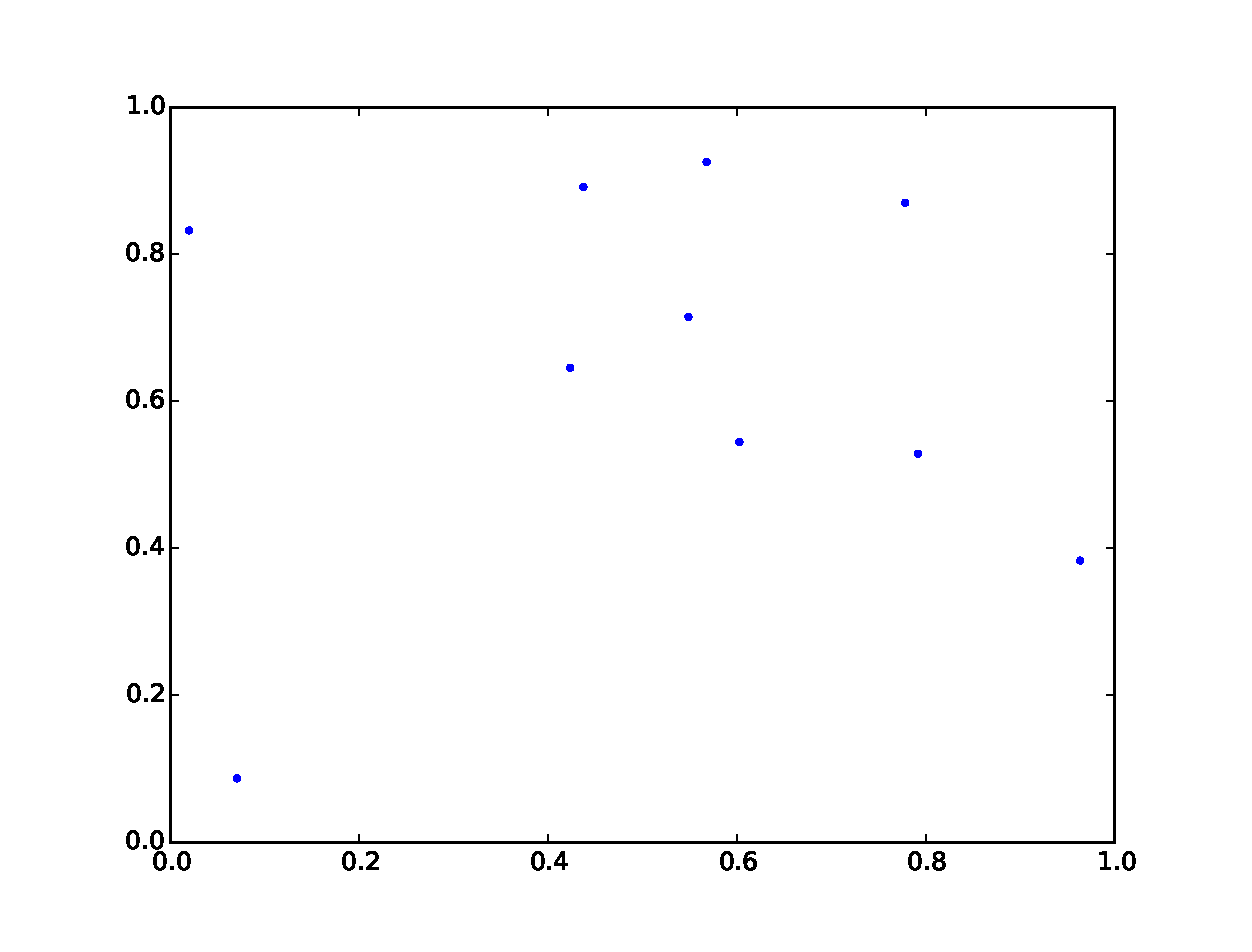
\includegraphics[width=\textwidth]{img/voroSites.eps}
      \end{center}
    \end{column}
    \begin{column}{0.5\textwidth}
      \begin{center}
        \includegraphics[width=\textwidth]<2->{img/voronoi.eps}
      \end{center}
    \end{column}
  \end{columns}
\end{frame}

\begin{frame}
  \frametitle{B-spline curves}
  \begin{center}
    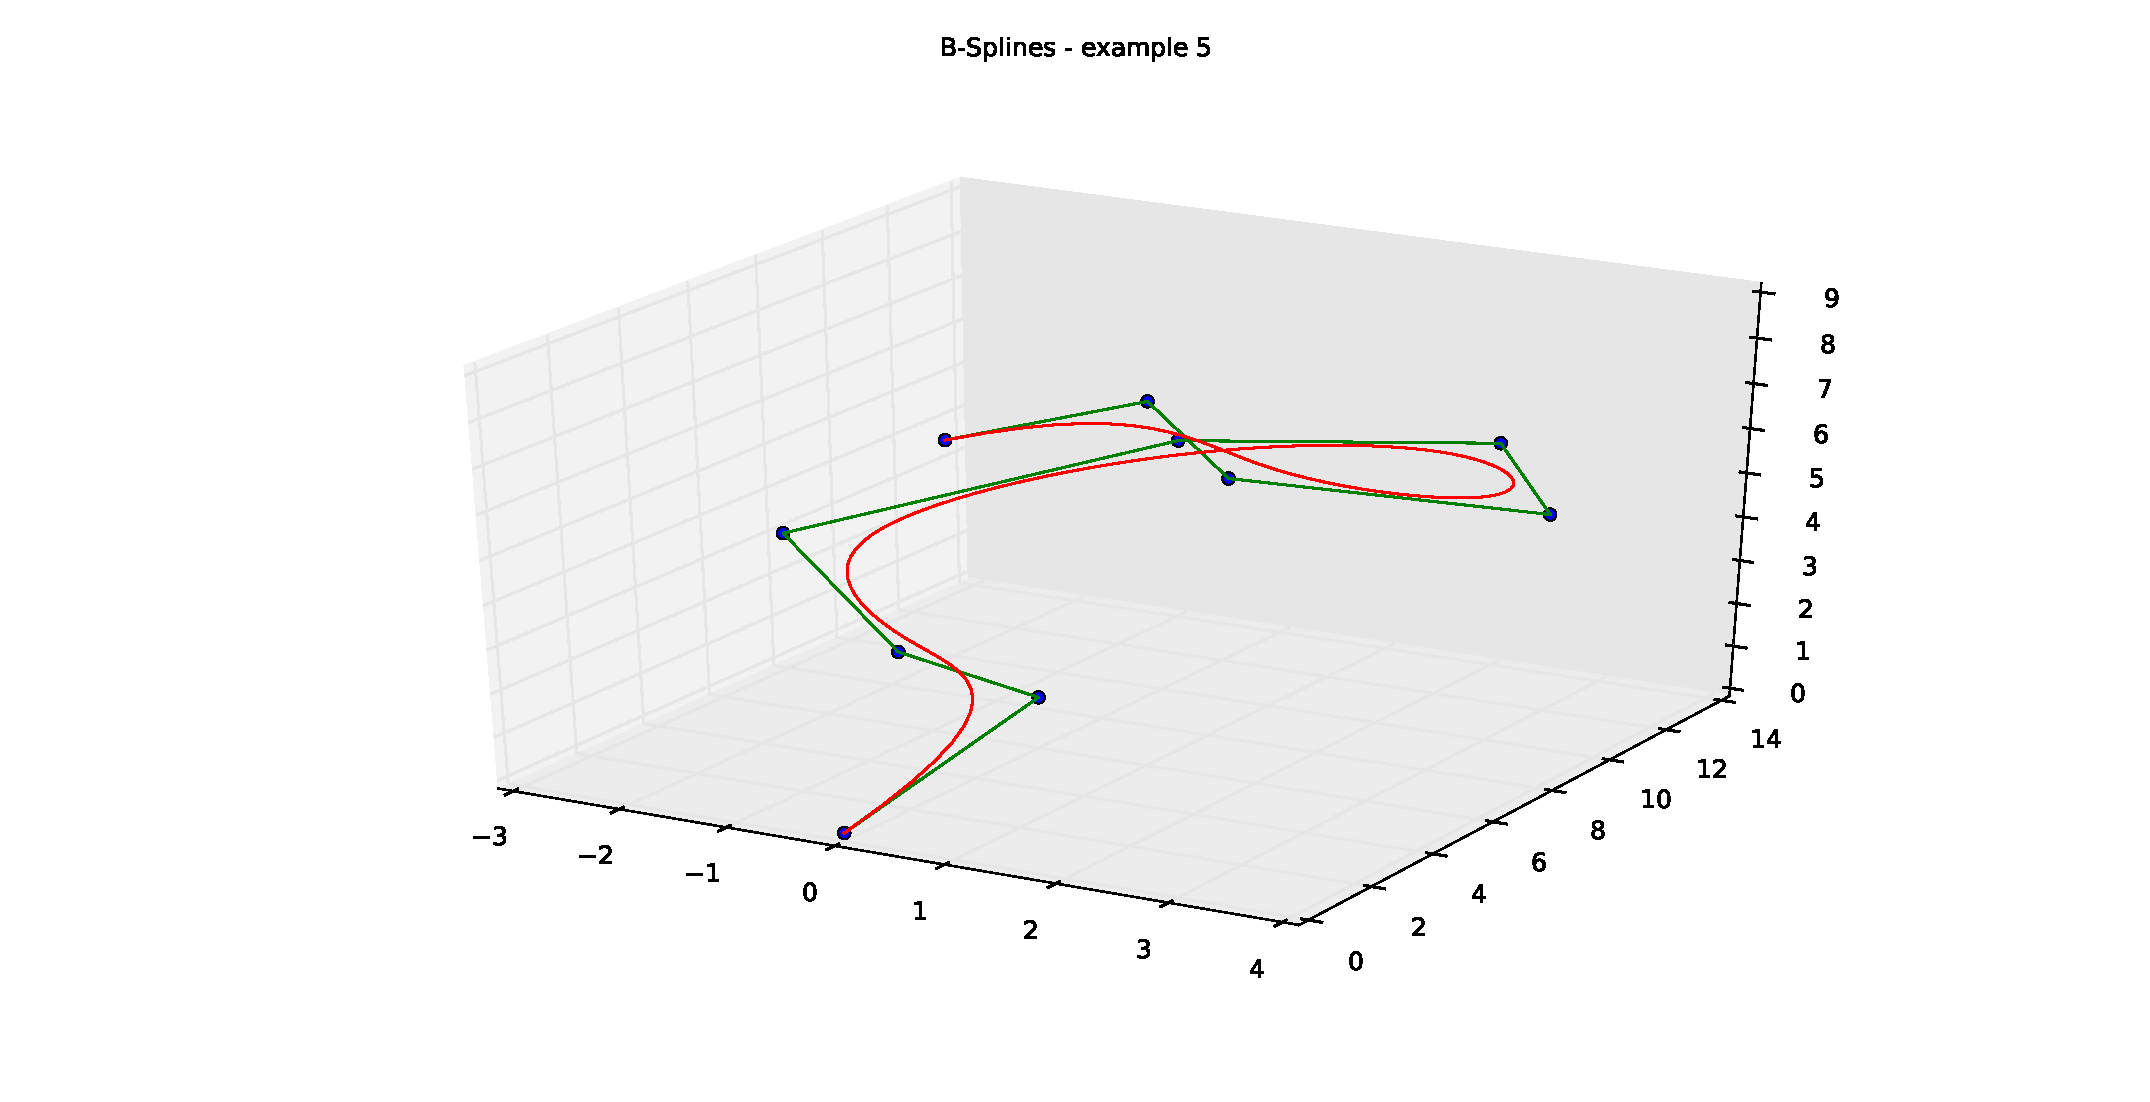
\includegraphics[width=0.8\textwidth, trim=110 30 50 50, clip]{img/bspline.eps}
  \end{center}
  \pause
  \begin{itemize}
  \item Piecewise polynomial \alert{parametric} curves
    $\ve{S}:[a,b]\rightarrow\mE^3$
    $\alert{\mathbf{S}(u)}=\sum_{i=0}^n\alert{\mathbf{v_i}}\cdot
    N_{i,m+1}(u)$\pause
  \item Prescribed \alert{regularity}\pause
  \item Follow the shape of a \alert{control poligon}\pause
  \item Can interpolate the
    \alert{extremes} of control polygon
  \end{itemize}
\end{frame}

\section{Background}

\begin{frame}
  \frametitle{Basic structure}
  \begin{center}
    \includegraphics[width=0.9\textwidth]<1>{img/scrEmpty.png}
    \includegraphics[width=0.9\textwidth]<2>{img/scrSites-a.png}
    \includegraphics[width=0.9\textwidth]<3>{img/scrSites-b.png}
    \includegraphics[width=0.9\textwidth]<4>{img/scrGraph-a.png}
    \includegraphics[width=0.9\textwidth]<5>{img/scrGraph-b.png}
  \end{center}
\end{frame}

\section{Implementation}

\begin{frame}
  \frametitle{Improvement}
  \begin{block}{Idea}
    \alert{Smoother} curve instead of polygonal chain
  \end{block}
  \pause
  \begin{itemize}
  \item Use a \alert{B-Spline} that \pause
    \begin{itemize}
    \item \alert{interpolate} the start and end\pause
    \item Shortest path as \alert{control polygon}
    \end{itemize}
  \end{itemize}
\end{frame}

\begin{frame}
  \frametitle{Problem}  
  \begin{itemize}
  \item \alert{Control polygon} obstacle-free by
    construction\pause
    \begin{itemize}
    \item (pruned of arcs that cross obstacles)\pause
    \end{itemize}
  \item \alert{Curve} not obstacle-free guaranteed\pause
  \end{itemize}
  \begin{center}
    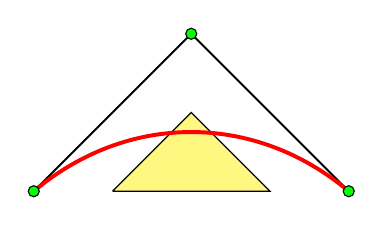
\begin{tikzpicture}
      \path[obstacle] (1,0) -- (2,1) -- (3,0) -- (1,0);
      \draw[controlPoly] (0,0) -- (2,2) -- (4,0);
      \draw[spline] (0,0) to [bend left=40] (4,0);

      \filldraw[controlVert] (0,0) circle (2pt);
      \filldraw[controlVert] (2,2) circle (2pt);
      \filldraw[controlVert] (4,0) circle (2pt);
    \end{tikzpicture}
  \end{center}
\end{frame}

\begin{frame}
  \frametitle{Solution}
  \begin{itemize}
  \item A \alert{B-Spline} of degree \alert{$m$} is contained
    inside the union of \alert{convex hulls} of
    \alert{$m+1$} consecutive vertices\pause
  \end{itemize}
  \begin{center}
    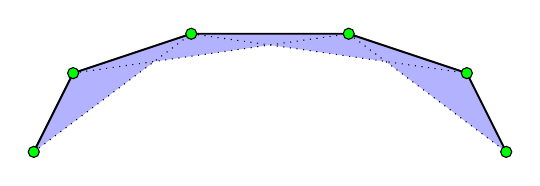
\begin{tikzpicture}
      \coordinate (a) at (0,0);
      \coordinate (b) at (0.5,1);
      \coordinate (c) at (2,1.5);
      \coordinate (d) at (4,1.5);
      \coordinate (e) at (5.5,1);
      \coordinate (f) at (6,0);

      \path[convexHull] (a) -- (b) -- (c) -- (a);
      \path[convexHull] (b) -- (c) -- (d) -- (b);
      \path[convexHull] (c) -- (d) -- (e) -- (c);
      \path[convexHull] (d) -- (e) -- (f) -- (d);

      \draw[convexHullBord] (a) -- (c);
      \draw[convexHullBord] (b) -- (d);
      \draw[convexHullBord] (c) -- (e);
      \draw[convexHullBord] (d) -- (f);

      \draw[controlPoly] (a) -- (b) -- (c) -- (d) -- (e) -- (f);
      \foreach \p in {a,b,c,d,e,f}
      \filldraw[controlVert] (\p) circle (2pt);
    \end{tikzpicture}
  \end{center}
  \pause
  \begin{block}{Idea}
    \begin{itemize}
    \item Use a \alert{quadratic} B-Spline to smooth path\pause
    \item \alert{Keep} triangles in control polygon \alert{obstacle-free}
    \end{itemize}
  \end{block}
\end{frame}

\begin{frame}
  \frametitle{First implementation}
  \begin{block}{Graph transformation (\alert{$G\rightarrow G_t$})}
    \begin{itemize}
    \item Triples \alert{$(a,b,c)$} of neighboring nodes in $G$ become
      nodes in $G_t$\pause
    \item Arcs in $G_t$ between triples in the form
      \alert{$(a,b,c)\rightarrow(b,c,d)$}\pause
      \begin{itemize}
      \item weighted with the distance of the edge
        \alert{$a\leftrightarrow b$} in $G$\pause
      \end{itemize}
    \end{itemize}
  \end{block}
  \begin{itemize}
  \item \alert{Prune} all the triples that intersect an obstacle\pause
  \item \alert{Shortest} path in the remaining triples\pause
  \end{itemize}
  \begin{center}
    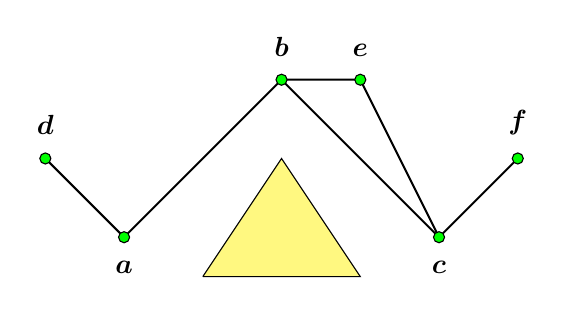
\begin{tikzpicture}
      \coordinate (D) at (-1,1);
      \coordinate (A) at (0,0);
      \coordinate (B) at (2,2);
      \coordinate (C) at (4,0);
      \coordinate (E) at (3,2);
      \coordinate (F) at (5,1);
      \path[obstacle] (1,-0.5) -- (2,1) -- (3,-0.5) -- (1,-0.5);
      \draw[controlPoly] (D) -- (A) -- (B) -- (C) -- (F);
      \draw[controlPoly] (B) -- (E) -- (C);

      \filldraw[controlVert] (D) circle (2pt);
      \filldraw[controlVert] (A) circle (2pt);
      \filldraw[controlVert] (B) circle (2pt);
      \filldraw[controlVert] (C) circle (2pt);
      \filldraw[controlVert] (E) circle (2pt);
      \filldraw[controlVert] (F) circle (2pt);

      \node[above=0.5em] at (D) {$\ve{d}$};
      \node[below=0.5em] at (A) {$\ve{a}$};
      \node[above=0.5em] at (B) {$\ve{b}$};
      \node[below=0.5em] at (C) {$\ve{c}$};
      \node[above=0.5em] at (E) {$\ve{e}$};
      \node[above=0.5em] at (F) {$\ve{f}$};
    \end{tikzpicture}
  \end{center}
\end{frame}

\begin{frame}
  \frametitle{Complexity}
  \begin{center}
    \begin{tabular}{|l|c|}
      \hline
      Description&Cost\\
      \hline
      \hline
      Creation of $G$&\eqCostGraph\\
      Pruning of $G$&\eqCostPruning\\
      Creation of $G_t$&\eqCostVt\\
      Pruning of $G_t$&\eqCostColl\\
      Routing in $G_t$& \eqCostDijkstraTriples\\
      \hline
      Total&\eqCostTotalOne\\
      Total ($k$ constant)&\eqCostTotalOneK\\
      \hline
    \end{tabular}
  \end{center}\pause
  \begin{itemize}
  \item Scene construction
    \begin{itemize}
    \item \alert{$\bigO(|O|^2)$}\pause
    \end{itemize}
  \item Routing
    \begin{itemize}
    \item \alert{$\bigO(|O|\log|O|)$}\pause
    \item (same of Dijkstra with constant degree)
    \end{itemize}
  \end{itemize}
\end{frame}

\begin{frame}
  \frametitle{Second implementation}
  \begin{block}{Reason}
    \begin{itemize}
    \item \alert{First} implementation interesting\pause
    \item[\xmark] but \alert{rejects} many paths
    \end{itemize}
  \end{block}\pause
  \begin{itemize}
  \item Shortest path on \alert{$G$}\pause
  \item \alert{Add} aligned control vertices when obstacle intersect triple
    \begin{center}
      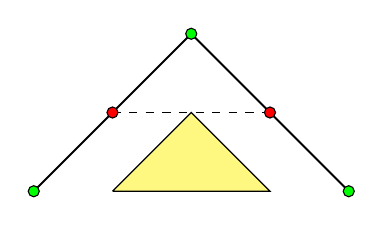
\begin{tikzpicture}
        \path[obstacle] (1,0) -- (2,1) -- (3,0) -- (1,0);
        \draw[controlPoly] (0,0) -- (2,2) -- (4,0);

        \filldraw[controlVert] (0,0) circle (2pt);
        \filldraw[controlVert] (2,2) circle (2pt);
        \filldraw[controlVert] (4,0) circle (2pt);

        \only<5->{
          \draw[controlPolyTract] (1,1) -- (3,1);
          \filldraw[controlVertHigh] (1,1) circle (2pt);
          \filldraw[controlVertHigh] (3,1) circle (2pt);
        }
      \end{tikzpicture}
    \end{center}
  \item<6-> new vertices \alert{easy} calculated after collision check
  \end{itemize}
\end{frame}

\begin{frame}
  \frametitle{Complexity}
  \begin{center}
    \begin{tabular}{|l|c|r|}
      \hline
      Description&Cost\\
      \hline
      \hline
      Creation of $G$&\eqCostGraph\\
      Pruning of $G$&\eqCostPruning\\
      Routing in $G$&\eqCostDijkstraG\\
      Clean path&\eqCostCleanPath\\
      \hline
      Total&\eqCostTotalTwo\\
      Total ($k$ costant)&\eqCostTotalTwoK\\
      \hline
    \end{tabular}
  \end{center}\pause
  \begin{itemize}
  \item Scene construction
    \begin{itemize}
    \item \alert{$\bigO(|O|^2)$}\pause
    \end{itemize}
  \item Routing
    \begin{itemize}
    \item \alert{$\bigO(|O|\log|O|+|P|\ |O|)$}
    \end{itemize}
  \end{itemize}
\end{frame}

\begin{frame}
  \frametitle{Increase degree}
  \begin{block}{Continuity}
    \begin{itemize}
    \item Using \alert{quadratic} B-Splines means \alert{$C^1$} continuity\pause
    \item[\xmark] Not enough
    \end{itemize}
  \end{block}\pause
  \begin{itemize}
  \item[\xmark] If \alert{increase} the B-Spline degree \alert{$\rightarrow$} convex hull not
    \alert{planar} anymore\pause
    \begin{itemize}
    \item convex hull formed of union of \alert{tetrahedra}\pause
    \end{itemize}
  \end{itemize}
  \begin{block}{Solution}
    \begin{itemize}
    \item \alert{Add} aligned vertices in control polygon\pause
      \begin{itemize}
      \item then \alert{increase} the degree
      \end{itemize}
    \end{itemize}
  \end{block}
\end{frame}

\begin{frame}
  \frametitle{Example: quadratic to quartic (m=2 $\rightarrow$ m=4)}
  \begin{itemize}
  \item Add \alert{2} vertices per edge
  \end{itemize}\pause
  \begin{center}
    \begin{tikzpicture}[scale=1.5]
      \coordinate (a1) at (0,2);
      \coordinate (a2) at (2,0.4);
      \coordinate (a3) at (4,1.6);
      \coordinate (a4) at (6,0);

      \coordinate (b1) at ($ (a1)!0.33!(a2) $);
      \coordinate (b2) at ($ (a2)!0.33!(a1) $);
      \coordinate (b3) at ($ (a2)!0.33!(a3) $);
      \coordinate (b4) at ($ (a3)!0.33!(a2) $);
      \coordinate (b5) at ($ (a3)!0.33!(a4) $);
      \coordinate (b6) at ($ (a4)!0.33!(a3) $);
      
      \only<-3>{
        \path[convexHull] (a1) -- (a2) -- (a3) -- (a1);
        \path[convexHull] (a2) -- (a3) -- (a4) -- (a2);
      
        \draw[convexHullBord] (a1) -- (a3);
        \draw[convexHullBord] (a2) -- (a4);
      }
      \only<4->{
        \path[convexHull] (a1) -- (b1) -- (b2) -- (a2) -- (b3) -- (a1);
        \path[convexHull] (b1) -- (b2) -- (a2) -- (b3) -- (b4) -- (b1);
        \path[convexHull] (b2) -- (a2) -- (b3) -- (b4) -- (a3) -- (b2);
        \path[convexHull] (a2) -- (b3) -- (b4) -- (a3) -- (b5) -- (a2);
        \path[convexHull] (b3) -- (b4) -- (a3) -- (b5) -- (b6) -- (b3);
        \path[convexHull] (b4) -- (a3) -- (b5) -- (b6) -- (a4) -- (b4);
      
        \draw[convexHullBord] (a1) -- (b3);
        \draw[convexHullBord] (b1) -- (b4);
        \draw[convexHullBord] (b2) -- (a3);
        \draw[convexHullBord] (a2) -- (b5);
        \draw[convexHullBord] (b3) -- (b6);
        \draw[convexHullBord] (b4) -- (a4);
      }

      \draw[controlPoly] (a1) -- (a2) -- (a3) -- (a4);
      \foreach \p in {a1,a2,a3,a4}
      \filldraw[controlVert] (\p) circle (2pt);

      \only<3->{
        \foreach \p in {b1,b2,b3,b4,b5,b6}
        \filldraw[controlVertHigh] (\p) circle (2pt);
      }
    \end{tikzpicture}
  \end{center}
\end{frame}

\begin{frame}
  \frametitle{Postprocessing}
  \begin{block}{Purpose}
    \begin{itemize}
    \item \alert{Simplify} the control polygon\pause
    \item \alert{Remove} useless turns
    \end{itemize}
  \end{block}\pause
  \begin{itemize}
  \item For each triple \alert{$(\ve{a},\ve{b},\ve{c})$} of
    consecutive points in path\pause
  \item If no obstacles intersect the triangle\uncover<5->{ 
      \alert{$\rightarrow$} the triple is simplified to a single edge
      \alert{$(\ve{a},\ve{c})$}}
  \uncover<6->{\item[\hmark] After simplification, \alert{new} neighbouring triples need to
    be obstacle-free}
  \end{itemize}
  \begin{center}
    \begin{tikzpicture}
      \coordinate (a) at (0,0);
      \coordinate (b) at (2,2);
      \coordinate (c) at (4,0);

      \only<-4>{
        \draw[controlPoly] (a) -- (b) -- (c);
      
        \filldraw[controlVert] (a) circle (2pt);
        \filldraw[controlVert] (b) circle (2pt);
        \filldraw[controlVert] (c) circle (2pt);
      }
      \only<5->{
        \draw[controlPoly] (a) -- (c);
      
        \filldraw[controlVert] (a) circle (2pt);
        \filldraw[controlVertHigh] (b) circle (2pt);
        \filldraw[controlVert] (c) circle (2pt);
      }

      \node[left=0.5em] at (a) {$\ve{a}$};
      \node[left=0.5em] at (b) {$\ve{b}$};
      \node[right=0.5em] at (c) {$\ve{c}$};
    \end{tikzpicture}
  \end{center}
 \end{frame}

\begin{frame}
  \frametitle{Optimization method}
  \begin{block}{Problem}
    \begin{equation*}
      \begin{aligned}
        & \underset{P}{\text{minimize}}
        & & \alpha\cdot \max_u[\kappa_{\ve{S}}(u)]+\beta\cdot
        \max_u[\tau_{\ve{S}}(u)]+\gamma\cdot len(\ve{S}) \\
        & \text{subject to}
        & & \left|\ve{S}(u)\cap \bigcup_{i\in I}obstacle_i\right| = 0
      \end{aligned}
    \end{equation*}\pause
  \end{block}
  \begin{itemize}
  \item \alert{Relax} constraint: $L(P,\lambda)=gain(P)+\lambda\cdot constraint(P)$\pause
  \item \alert{Saddle} point $L(P^*,\lambda)\leq L(\alert{P^*},
    \alert{\lambda^*})\leq L(P,\lambda^*)$\pause
  \item \alert{Simulated annealing} finds saddle point that minimize gain
  \end{itemize}
\end{frame}

\begin{frame}
  \frametitle{Used technologies}
  \begin{center}
    \visible<1->{
\includegraphics[width=4cm]{img/python3.png}}\\[1cm]
    \visible<2->{
\includegraphics[width=4cm]{img/scipy.png}}\\[1cm]
    \visible<3->{
\includegraphics[width=4cm]{img/vtk.png}}
  \end{center}
\end{frame}

\begin{frame}
  \frametitle{Future improvements}
  \begin{itemize}
  \item Change underlying \alert{structure}\pause
    \begin{itemize}
    \item visibility graph\pause
    \item rapidly exploring random tree (RRT)\pause
    \item other \dots\pause
    \end{itemize}
  \item Improve \alert{degree} increase\pause
    \begin{itemize}
    \item without \alert{aligned} vertices\pause
    \item like second solution but with quadruple/quintuples
      of vertices\pause
    \end{itemize}
  \item Improve \alert{postprocessing}\pause
    \begin{itemize}
    \item make a \alert{symmetric} algorithm\pause
    \end{itemize}
  \item Another \alert{optimization} process\pause
    \begin{itemize}
    \item output of other solutions as initial state\pause
    \item moves in a restricted space
    \end{itemize}
  \end{itemize}
\end{frame}

\begin{frame}
  \begin{center}
	\textbf{\calligra\Huge The End.}\\
  
\includegraphics[width=5cm]{img/ornament.eps}\\[1cm]
	\pause
	{\huge\calligra Questions?\pause{} Thank you!}
  \end{center}
\end{frame}

\appendix

\begin{frame}
  \frametitle{B-spline curves details}
  \begin{itemize}
  \item Degree \alert{$m$}\pause
  \item Extended \alert{partition} (of parametric
    space \alert{$[a,b]$})
    $$
    T=\{t_0,\dots,t_{m-1},\alert{t_{m}},\dots,\alert{t_{n+1}},t_{n+2},\dots,t_{n+m+1}\}
    $$
    {\tiny
      $$
      t_0\leq\dots\leq t_{m-1}\leq t_{m}\alert{(\equiv a)} <\dots<
      t_{n+1}\alert{(\equiv b)} \leq t_{n+2}\leq\dots\leq t_{n+m+1}
      $$
    }\pause
  \item \alert{$n+1$ basis} (of $S_{m,\tau}=P_{m,\tau}\cap C^{m-1}$)
    {\tiny
      \begin{align*}
        \alert{N_{i,1}(u)} &=
                     \begin{cases}
                       1,\quad \mbox{if}\quad t_i\leq t<t_{i+1}\\
                       0,\quad \mbox{otherwise}\qquad\qquad\qquad i=0,\dots,n+m
                     \end{cases}\\
        \alert{N_{i,r}(u)} &= \omega_{i,r-1}(u)\cdot \alert{N_{i,r-1}(u)}\ +\
                     (1-\omega_{i+1,r-1}(u))\cdot \alert{N_{i+1,r-1}(u)}\\
                   &\pushright i=0,\dots,n+m+1-3,\ r=2,\dots,m+1
      \end{align*}
    }
    {\tiny
      $$
      \omega_{i,r}(u) = \begin{cases}
        \frac{t-t_i}{t_{i+r}-t_i},&\mbox{if }t_i\neq t_{i+r}\\
        0, &\mbox{otherwise}
      \end{cases}
      $$
    }\pause
  \item B-spline curve $\ve{S}:[a,b]\subset\mR\rightarrow\mE^d$
    $$
    \alert{\mathbf{S}(u)}=\sum_{i=0}^n\alert{\mathbf{v_i}}\cdot N_{i,m+1}(u)
    $$
  \end{itemize}
\end{frame}

\begin{frame}
  \frametitle{Useful properties of B-spline curves}
  \begin{itemize}
  \item \alert{Interpolates} extremes if $t_0=\dots =t_{m}$ and $t_{n+1}=\dots
    =t_{n+m+1}$\pause
  \item \alert{Continuity} $C^{m-1}$ between polynomials\pause
  \item Contained in \alert{convex hulls} of 
    \alert{$m+1$} consecutive vertices
    \begin{center}
      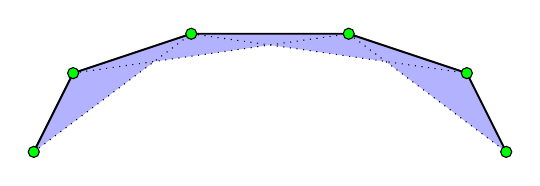
\begin{tikzpicture}
        \coordinate (a) at (0,0);
        \coordinate (b) at (0.5,1);
        \coordinate (c) at (2,1.5);
        \coordinate (d) at (4,1.5);
        \coordinate (e) at (5.5,1);
        \coordinate (f) at (6,0);
        
        \path[convexHull] (a) -- (b) -- (c) -- (a);
        \path[convexHull] (b) -- (c) -- (d) -- (b);
        \path[convexHull] (c) -- (d) -- (e) -- (c);
        \path[convexHull] (d) -- (e) -- (f) -- (d);
        
        \draw[convexHullBord] (a) -- (c);
        \draw[convexHullBord] (b) -- (d);
        \draw[convexHullBord] (c) -- (e);
        \draw[convexHullBord] (d) -- (f);
        
        \draw[controlPoly] (a) -- (b) -- (c) -- (d) -- (e) -- (f);
        \foreach \p in {a,b,c,d,e,f}
        \filldraw[controlVert] (\p) circle (2pt);
      \end{tikzpicture}
    \end{center}\pause
  \item Touches segment between \alert{$m$ aligned}
    vertices\pause
  \item Lays in segment between \alert{$m+1$ aligned} vertices\pause
  \end{itemize}
  \begin{align*}
    \kappa(u) &= \frac{\norm{\dot{\ve{S}}(u)\wedge\ddot{\ve{S}}(u)}}{{\norm{\dot{\ve{S}}(u)}}^3}\\
    \tau(u) &= \frac{\det\left[\dot{\ve{S}}(u),\ddot{\ve{S}}(u),\dddot{\ve{S}}(u)\right]}{\norm{\dot{\ve{S}}(u)\wedge\ddot{\ve{S}}(u)}} = \frac{\left(\dot{\ve{S}}(u)\wedge\ddot{\ve{S}}(u)\right)\cdot\dddot{\ve{S}}(u)}{\norm{\dot{\ve{S}}(u)\wedge\ddot{\ve{S}}(u)}}
  \end{align*}
\end{frame}

\begin{frame}
  \frametitle{Background}
  \begin{block}{Main problem}
    \alert{Path planning} from a \alert{start} point to an \alert{end}
    point in 3D space with obstacles using \alert{Voronoi} diagrams.
  \end{block}\pause
  \begin{enumerate}
  \item Distribute \alert{points} in obstacles surfaces
    \begin{itemize}
    \item and bounding box\pause
    \end{itemize}
  \item \alert{Voronoi} diagram using those points\pause
  \item Transform Voronoi diagram in \alert{graph}
    \begin{itemize}
    \item cells \alert{vertices} $\rightarrow$ \alert{nodes}
    \item cells \alert{edges} $\rightarrow$ \alert{arcs} (infinite edges
      ignored)\pause
    \end{itemize}
  \item \alert{Prune} arcs that cross obstacles\pause
  \item Attach \alert{start} and \alert{end}\pause
  \item Shortest path from start to end
    \begin{itemize}
    \item \alert{Dijkstra}'s algorithm
    \end{itemize}
  \end{enumerate}
\end{frame}

\begin{frame}
  \frametitle{Intersection segment-triangle}
  \begin{center}
    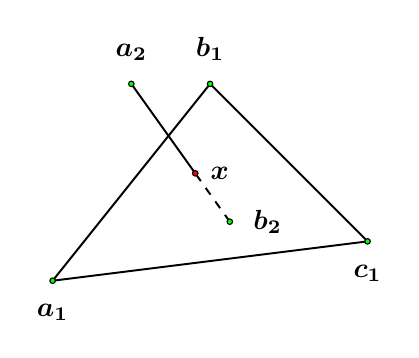
\begin{tikzpicture}[scale=0.5]
      \coordinate (A1) at (0,0);
      \coordinate (B1) at (4,5);
      \coordinate (C1) at (8,1);

      \coordinate (cut1) at (barycentric cs:A1=0.8,B1=0.,C1=0.2);
      \coordinate (cut2) at (barycentric cs:A1=0.,B1=0.8,C1=0.2);

      \coordinate (A2) at (2,5);    
      \coordinate (B2) at (4.5,1.5);

      \coordinate (X) at (intersection of cut1--cut2 and B2--A2);

      \draw[poly] (A1) -- (C1) -- (B1) -- (A1);
      \draw[poly] (A2) -- (X);
      \draw[polyTract] (B2) -- (X);

      \foreach \p in {A1,B1,C1,A2,B2}
      \filldraw[vertex] (\p) circle (2pt);

      \filldraw[intersection] (X) circle (2pt);

      \node[below=0.5em] at (A1) {$\ve{a_1}$};
      \node[above=0.5em] at (B1) {$\ve{b_1}$};
      \node[below=0.5em] at (C1) {$\ve{c_1}$};
      \node[above=0.5em] at (A2) {$\ve{a_2}$};
      \node[right=0.5em] at (B2) {$\ve{b_2}$};
      \node[right=0.2em] at (X) {$\ve{x}$};
    \end{tikzpicture}
  \end{center}
  \tiny
  \begin{equation*}
    \begin{cases}
      \alpha \ve{a_2} + \beta\ve{b_2}=\gamma\ve{a_1}+\delta\ve{b_1}+\zeta\ve{c_1} \\
      \alpha + \beta = 1\\
      \gamma + \delta +\zeta=1
    \end{cases}
  \end{equation*}
  \begin{equation*}
    \begin{cases}
      \alpha \ge 0\\
      \beta \ge 0\\
      \gamma \ge 0\\
      \delta \ge 0\\
      \zeta \ge 0.
    \end{cases}
  \end{equation*}
\end{frame}
\end{document}

%%% Local Variables:
%%% mode: latex
%%% TeX-master: t
%%% End:
